%%%%%%%%%%%%%%%%%%%%%%%%%%%%%%%%%%%%%%%%%
% Simple Article
% Integrated article template with simple for make4ht
% LaTeX Class
% Version 1.0 (10/11/20)
%
% This class originates by:
% Vel and  Nicolas Diaz
%
% Authors:
% Muhammad Uliah Shafar
%
%
% Free License:
%
%
%%%%%%%%%%%%%%%%%%%%%%%%%%%%%%%%%%%%%%%%%
\documentclass[11pt]{udthesis} % Font size (can be 10pt, 11pt or 12pt)

%----------------------------------------------------------------------------------------
%	TITLE SECTION
%----------------------------------------------------------------------------------------
% MAIN TITLE SECTION
\title{
\textbf{Lorem Ipsum Lorem Ipsum \\
Lorem Ipsum Lorem Ipsum Lorem Ipsum} \\
\textbf{{Lorem Ipsum Lorem Ipsum \\}}
} % Title and subtitle
%\date{\textbf{\DTMtoday}}
\date{\textbf{\today}}
\author{
\begin{tabular}{@{}ll@{}}
	Nama & : Muhammad Uliah Shafar\\
	NIM & : 21020119420029\\
\end{tabular}
}

%----------------------------------------------------------------------------------------
% OTHER TITLE SECTION

%\title{\textbf{Sistem Sarana dan Prasarana Jl. Pinggir Laut} \\ {\Large\itshape Infrastructure of Waterfront Parepare City}} % Title and subtitle

%\author{\textbf{Uliah Shafar} \\ \textit{Universitas Diponegoro}} % Author and institution

%\date{\today} % Date, use \date{} for no date

%----------------------------------------------------------------------------------------



\begin{document}

%----------------------------------------------------------------------------------------
%	ESSAY BODY
%----------------------------------------------------------------------------------------
\section{Pendahuluan}

Tepi laut merupakan sebuah ruang perkotaan yang sangat memerlukan pengembangan secara terus menerus \citep{shamsuddin2013}. Ruang ini mempunyai sejumlah karakteristik-karakteristik yang unik oleh karena air merupakan sumber kehidupan \citep{yassin2010}. Pengembangan tepi laut yang sukses mempertimbangkan sejumlah aspek yaitu keberagaman, interaksi komunitas, kenyamanan dan keamanan, lingkungan dan keberlanjutan \citep{hussein2014}. Pengembangan yang sukses oleh tepi laut akan mengantarkan masyarakat menuju ke kawasan tepi laut dari pusat kota \citep{hoyle2001}.

Pembahasan terkait pengembangan tepi laut belakangan ini menjadi topik yang hangat di Indonesia. Terdapat sejumlah pengembangan yang terjadi di sejumlah daerah seperti proyek reklamasi di Makassar dan Manado \citep{andi2017,fhuh2017,tungka2012}, desain lanskap tepi laut di sungai Cikapundung \citep{ainy2016}, dan pengembangan ulang tepi laut tahun 1995 sepanjang 32 km di Jakarta \citep{pramesti2017}. Kota Parepare menjadi salah satu penggagas pengembagan tepi laut sebagai tempat wisata. Salah satu pengembangan terjadi pada daerah pantai senggol \citep{tri2020}.

Tepi laut senggol merupakan daya tarik wisata masyarakat kota Parepare sejak lama. Orang-orang dapat menikmati pemandangan yang indah dan ditemani dengan makanan-makanan khas pedagang kaki lima. Selain itu, mereka juga dapat berenang di laut. Aktivitas-aktivitas tersebut yaitu interaksi dengan air menjadi bagian terpenting dalam pengembangan tepi laut \citep{davidowich1998}. \cite{eldeeb2015} menambahkan penggunaan beragam akan berkontribusi terhadap kesuksesssan sebuah tepi laut.

Pada dasarnya, tepi laut merupakan sebuah ruang yang dapat meningkatkan kualitas hidup seseorang dengan cara memenuhi kebutuhan masyarakat \citep{kim2012}.
Untuk memenuhi kebutuhan tersebut secara efektif sehingga dapat meningkatkan kualitas hidup penggunanya, maka pemangku kebijakan dan perencana kota dalam mendesain ruang publik memerlukan pemahaman preferensi terhadap ruang publik yang lebih baik \citep{madureira2018}.
Preferensi terhadap ruang adalah ungkapan keinginan seseorang terhadap suatu ruang \citep{zhang2006}. Ungkapan keinginan ini melekat atau ditimbulkan oleh sebuah elemen ruang perkotaan \citep{knox2014}. Menurut \cite{alves2008}, elemen ruang merupakan bagian fisik dari sebuah ruang publik yang termasuk dalam tatanan ruang publik itu sendiri.

Penelitian terkait preferensi pengunjung terhadap ruang publik di sekitar kawasan tepi laut masih kurang. Hanya ada beberapa penelitian yang membahas preferensi terhadap taman kota \citep{alves2008,devysandra2012,dwiputra2017,madureira2018}, taman publik untuk umum  \citep{grilli2020}, dan ruang publik kampus \citep{zhang2006}. Sehingga penelitian ini diharapkan mampu melengkapi kekurangan studi preferensi tersebut.

Penelitian ini, selain membahas preferensi terhadap ruang publik secara umum, juga akan mengkaji latar belakang pengguna ruang publik. Tujuannya untuk memberikan gambaran bagaimana preferensi masyarakat lokal. Ini penting karena preferensi masyarakat dalam suatu wilayah dapat berbeda \citep{madureira2018}.

Dalam kurung waktu kurang dari satu dekade, pengembangan kawasan tepi laut Senggol Parepare selesai. Pengembangan ini menghasilkan dua jenis ruang yang berbeda. Untuk memudahkan, penelitian ini menyebut ruang yang satu sebagai ruang A, sedangkan ruang lainnya sebagai ruang B. Kedua ruang ini memiliki sejumlah perbedaan dari segi elemen-elemen ruang, aktivitas, dan lain-lain.

Ruang A lebih dikenal dengan tatanan dan elemen buatan yang mewah dan lengkap. Sedangkan ruang B lebih dikenal dengan tatanan dan elemen yang terlihat lebih alami dengan sedikit elemen buatan. Sehingga, kedua ruang ini memunculkan kondisi yang kontras yang membuat orang berpeluang untuk memilih satu ruang daripada lainnya. Kondisi ini dalam kurung waktu tertentu akan menghasilkan ketidakselarasan dimana ruang satu akan terlihat lebih berhasil dalam menarik pengunjung daripada ruang lainnya. Ketidakselaran jumlah pengunjung yang mungkin terjadi ini akan membuat kawasan secara keseluruhan tidak optimal \citep{sari2015}. Menurut \cite{madureira2018}, pemahaman preferensi akan menjawab permasalahan tersebut dengan cara menjelaskan kebutuhan-kebutuhan pengunjung.



\section{Metode Penelitian}
\label{sub:metpen}

Penelitian ini bertujuan untuk menganalisis preferensi pengunjung terhadap ruang di tepi laut Senggol. Tujuan tersebut dapat tercapai dengan menerapkan pendekatan penelitian. Penelitian ini menerapkan pendekatan kualitatif dan kuantitatif \textit{(mixed-method)}. Menurut \cite{creswell2016}, pendekatan kualitatif merupakan gambaran keseluruhan dari sebuah fenomena yang diambil dari pemahaman dan penglihatan secara langsung sebuah fenomena dalam objek penelitian dengan sejumlah sumber yang tersedia. Dalam penelitian ini, fenomena tersebut adalah kecenderungan pengunjung dalam memilih ruang. Sedangkan pendekatan kuantitatif digunakan untuk meneliti populasi atau sampel tertentu berdasarkan variabel penelitian. Lebih lanjut, untuk menilai frekuensi munculnya variabel yang menarik di setiap ruang, maka penelitian ini menerapkan desain analitik dengan pendekatan \textit{cross sectional} sebagai analisis data.

Penelitian ini berlokasi di kawasan tepi laut Senggol di Kota Parepare yang terbentang dari pelabuhan Nusantara hingga Pasar Senggol (lihat gambar \ref{fig:lokzi}). Penelitian ini dilaksanakan setiap hari pada jam 6 - 10 pagi dan 6 - 9 malam karena pada waktu ini menunjukkan keramaian di objek penelitian. Adapun pengumpulan data terbagi atas dua macam data yakni data primer dan sekuder. Pertama, Data primer adalah data yang diambil dari hasil kuesioner yang berdasarkan variabel penelitian. Terakhir, data sekunder merupakan informasi yang telah tersedia oleh pihak atau instansi lain.

\begin{figure}[htpb]
    \centering
    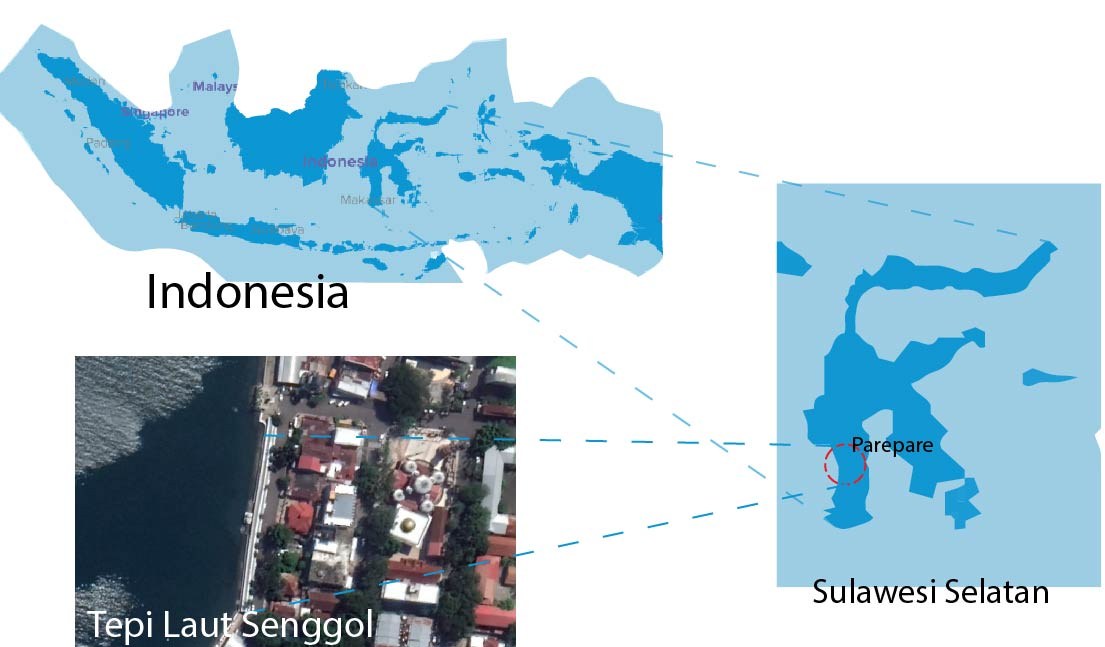
\includegraphics[width=0.86\textwidth]{figures/lokzi}
    \caption{Lokasi Kota Parepare}
    \caption*{Sumber: Dokumentasi, 2022}
    \label{fig:lokzi}
\end{figure}

Penelitian ini menganalisis data dari hasil survei kuesioner terkait preferensi pengunjung yang disertai dengan alasan memilih elemen-elemen yang disukai. Sebelum menganalisis kedua data yang bersifat kualitatif dan kuantitatif, maka peneliti melakukan reduksi data. Setelah itu, peneliti menganalisis data berdasarkan kedua jenis data tersebut.
Untuk data yang berjenis kualitatif seperti kecenderungan dan deskripsi, peneliti mempelajari makna tema-tema yang terdapat dalam teks responden.
Hasil analisis ini menggambarkan data yang dikategorisasikan sesuai dengan kriteria yang didapatkan.
Untuk data yang berjenis kuantitatif, peneliti memahami karakteristik setiap variabel dengan menggunakan pendekatan \textit{cross-sectional}. Hasilnya mengilustrasikan keragaman preferensi terhadap ruang berdasarkan aspek dan elemen ruang serta latar belakang diantara responden atau kelompok.

Kriteria pada penelitian ini terangkum dalam variabel penelitian. Penelitian ini menggunakan variabel tunggal yang hanya memunculkan variabel untuk di deskripsikan faktor atau unsur didalam setiap gejala dalam variabel tersebut. Variabel penelitian secara detil dapat dilihat pada tabel \ref {tab:varpar}.
\newpage

\begin{table}[hp!]
    \small
    \centering
    \caption{Variabel penelitian}
    \label{tab:varpar}
    \begin{tabular}{p{.23\textwidth}p{.33\textwidth}m{.33\textwidth}}
\toprule
\textbf{Variabel} & \textbf{Sub-Variabel} & \textbf{Indikator}  \\
\midrule
\multirow{5}{*}{Aksesibilitas\tikzmark{ak}} & \tikzmark{jp}Jumlah pohon & Sedikit pohon\\
& & Beberapa pohon\\
\cmidrule{2-3}

& \multirow{2}{*}{\tikzmark{bp}Bentuk pohon} & Cukup rindang\\
& & Rindang\\
\cmidrule{2-3}

& \multirow{2}{*}{\tikzmark{lj}Lebar jalan} & 1-3m\\
\multirow{5}{*}{Keamanan\tikzmark{ke}}& & 3m\\
\cmidrule{2-3}


& \multirow{3}{*}{\tikzmark{pj}Permukaan jalan} & Paving\\
& & Aspal \\
& & Tanah \\
\cmidrule{2-3}

& \multirow{2}{*}{\tikzmark{wb}Warna bunga/tanaman} & satu atau dua warna\\
& & tiga atau lebih warna\\
\cmidrule{2-3}

& \multirow{2}{*}{\tikzmark{jk}Jenis kursi} & Kursi bergerak \\
& & Kursi dinding \\
\cmidrule{2-3}

\multirow{5}{*}{Estetika\tikzmark{es}}& \multirow{2}{*}{\tikzmark{tc}Tingkat cahaya} & Sedang\\
& & Tinggi\\
\cmidrule{2-3}

& \multirow{2}{*}{\tikzmark{oe}Orientasi elemen} & Membelakangi laut\\
& & Menghadap laut\\
\cmidrule{2-3}

& \multirow{2}{*}{\tikzmark{tw}Tempat wisata air} & Tempat memancing\\
& & Tempat berenang\\
\cmidrule{2-3}

\multirow{5}{*}{Fasilitas\tikzmark{fa}}& \multirow{2}{*}{\tikzmark{bap}Bangunan penunjang} & Stan \\
& & Kedai\\
\cmidrule{2-3}

& \multirow{2}{*}{\tikzmark{ea}Elemen air} & Laut tenang\\
& & Laut berombang\\
\bottomrule
\end{tabular}
\end{table}


\begin{tikzpicture}[overlay,remember picture,shorten >=.5pt,shorten <=.5pt, transform canvas={yshift=.25\baselineskip}]
    \draw [->] ({pic cs:ak}) -- ({pic cs:lj});
    \draw [->] ({pic cs:ak}) -- ({pic cs:pj});
    \draw [->] ({pic cs:ke}) -- ({pic cs:bp});
    \draw [->] ({pic cs:ke}) -- ({pic cs:pj});
    \draw [->] ({pic cs:es}) -- ({pic cs:jp});
    \draw [->] ({pic cs:es}) -- ({pic cs:wb});
    \draw [->] ({pic cs:es}) -- ({pic cs:ea});
    \draw [->] ({pic cs:fa}) -- ({pic cs:bp});
    \draw [->] ({pic cs:fa}) -- ({pic cs:jk});
    \draw [->] ({pic cs:fa}) -- ({pic cs:lj});
    \draw [->] ({pic cs:fa}) -- ({pic cs:oe});
    \draw [->] ({pic cs:fa}) -- ({pic cs:tw});
    \draw [->] ({pic cs:fa}) -- ({pic cs:bap});
    \draw [->] ({pic cs:sd}) -- ({pic cs:g});
    \draw [->] ({pic cs:sd}) -- ({pic cs:u});
    \draw [->] ({pic cs:sd}) -- ({pic cs:s});
    \draw [->] ({pic cs:sd}) -- ({pic cs:p});
\end{tikzpicture}



%----------------------------------------------------------------------------------------
%	BIBLIOGRAPHY
%----------------------------------------------------------------------------------------

\bibliographystyle{apacite}
\bibliography{biblioold.bib}

\end{document}
